% !TEX ROOT = ../ersti.tex


\begin{figure*}[b]
    \centering
    \begin{subfigure}{.24\textwidth}
	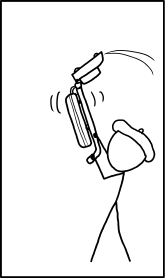
\includegraphics[height=5cm]{bilder/vacuum_1.png}
    \end{subfigure}
    \begin{subfigure}{.24\textwidth}
	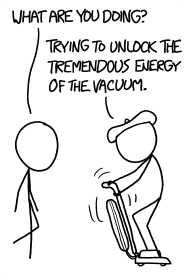
\includegraphics[height=5cm]{bilder/vacuum_2.png}
    \end{subfigure}
    \begin{subfigure}{.24\textwidth}
	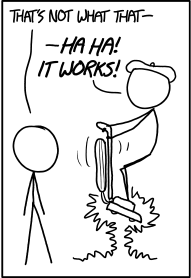
\includegraphics[height=5cm]{bilder/vacuum_3.png}
    \end{subfigure}
    \begin{subfigure}{.24\textwidth}
	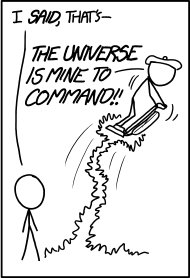
\includegraphics[height=5cm]{bilder/vacuum_4.png}
    \end{subfigure}
\end{figure*}

\section{Semesterticket}
Seit mehr als 20 Jahren hat Heidelberg ein Semesterticket, das es den Studierenden ermöglicht, kostengünstig den öffentlichen Nahverkehr zu nutzen. Zur Einführung waren alle Beteiligten von der großen Resonanz überrascht und das Ticket entwickelte sich zu einem Erfolg. Enorme Preissteigerungen von 127\% in der bisherigen Geschichte haben jedoch dazu geführt, dass die Nutzerzahlen deutlich sinken und das Semesterticket von vielen als unattraktiv und überteuert wahrgenommen wird.

Ein Semesterticket muss stets eine Vielzahl von Interessen befriedigen. Es sollte ein attraktives und günstiges Ticket im Stadtbereich sein und das direkte Umfeld des Hochschulstandortes erschließen. Des Weiteren ist es wünschenswert, die ländliche Region anzubinden und den dort wohnhaften Studierenden einen Umzug und hohe Mieten zu ersparen. Neben dem täglichen Pendelverkehr ist die Heimreise zum elterlichen Wohnsitz ebenfalls für eine Vielzahl von Studierenden ein Grund, ein Semesterticket zu erwerben.

Das aktuelle Semesterticket in Heidelberg wird vom Verkehrsverbund Rhein-Neckar (VRN) angeboten und gilt für ein Semester. Es berechtigt zu Fahrten im gesamten Tarifgebiet außer der Westpfalz\footnote{\url{http://www.vrn.de/vrn/einfach-ankommen/linienplaene/stadt-und-netzlinienplaene/gesamtliniennetzplan/index.html}} -- „einem Schlauch von Polen nach Frankreich“\footnote{Zitat aus der Semesterticket Umfrage der FSK im Jahr 2013}. Die Ausdehnung ist in Ost-West Richtung sehr weitreichend, in Nord-Süd Richtung ist jedoch nach 20\,km von Heidelberg aus Schluss. Das Semesterticket finanziert sich aus einem Kaufpreis von aktuell \EUR{\semesterticket} und einem solidarischen Sockelbeitrag von \EUR{\sockelbeitrag}, den alle Studierenden mit dem Studierendenwerksbeitrag bei der Rückmeldung zahlen müssen -- auch wenn sie das Ticket nicht nutzen. Eine Heidelberger Besonderheit bei der Sockelfinanzierung ist, dass sie es allen Studierenden ermöglicht, unter der Woche ab 19 Uhr und am Wochenende und Feiertagen ganztags innerhalb des VRN-Gebietes kostenlos mit Bus und Bahn fahren zu können -- der Studiausweis gilt dabei als Fahrschein.

Seit Jahren verhandeln das Verkehrsreferat der Studierendenvertretung und das Studierendenwerk unermüdlich mit dem VRN über einen neuen Vertrag. Die Studis fordern ein Ende der enormen Preissteigerungen, um auch in Zukunft mit dem Semesterticket ein günstiges Nahverkehrsangebot zu gewährleisten. Da der VRN jedoch weiter an Preissteigerungen von ca. 10\% pro Jahr festhalten will, stand das Semesterticket vor dem Aus. Zwischendurch kam der Kommunalwahlkampf in Heidelberg den Studis zu Gute, aber trotz massiven Drucks aus der Politik und Zuschüssen durch den Gemeinderat ist das Semesterticket nach wie vor recht teuer und der VRN wird die Preise weiterhin regelmäßig erhöhen.

Mittlerweile steigt das Semesterticket im Preis jedes Semester. Der StuRa und vor allem dessen Verkehrsreferat setzt sich dafür ein, die Preise so gering wie möglich zu halten, was kein leichtes Unterfangen ist.

Weitere Informationen zu den Verhandlungen und dem Semesterticket findest du auf der StuRa-Seite\footnote{\url{http://www.stura.uni-heidelberg.de/semesterticket}}.
